\Chapter{Tervezés}

\Section{A programozási nyelv kiválasztása}

A program HTML, JavaScript nyelven fog íródni, HTML5 Canvas használatával. Az objektum orientált programozáshoz igazodva osztályokat fog használni. Ezekből 3 darabra lesz szükség mindkét program esetében. 

\Section{Megjelenítés elkészítésének lépései} 

Az egyik program esetében először el kell dönteni, hogy hogyan rajzoljuk ki a köröket. Ehhez 2 módszer is szóba jöhet. Aztán ezek közül ki kell választani, nyilván azt amelyik gyorsabbnak bizonyul. 
A másik program esetében a négyzetek kirajzolásán kell gondolkoznunk. Itt nem merült fel 2 módszer, mivel a körök esetében már vizsgáltunk gyorsaságot, valószínűleg a négyzetek esetében is ugyanazt a módszert találnánk gyorsabbnak.

\Section{Mozgatás}

Ha kész a megjelenítés, akkor jöhet a mozgatás. Aminél számításba kell venni, hogy gravitációnak kell a körökre/négyzetekre hatnia  és, hogy minden részecskének van súlya, sűrűsége. Illetve a képfrissítéssel is számolnunk kell \cite{game}.

\Section{Ütközések}


\textbf{Fal}
Ha megvan a mozgás utána jöhet az ütközések vizsgálata, aminél érdemes először a falakkal kezdeni. Mind a 4 falra vizsgálnunk kell az ütközéseket \cite{bounce}. Itt a körök esetében számításba kell venni a sugarat is. A négyzetek esetében pedig a magasságot meg a szélességet. 

\textbf{Részecskék}
Aztán ha az megvan jöhet a részecskék egymás közötti ütközése is. Egymás között is az összes részecskére érdemes nézni az ütközéseket. Itt is számolnunk kell a részecskék súlyával, méretével. 

\Section{Akadályok}

Amennyiben már ütközések kezeléséhez szükséges kódrészek is megvannak, jöhetnek az akadályok, ami nekünk valószínűleg egy pohár lesz \cite{collision}. Aztán erre/ezekre az akadályokra is szükséges megírni az ütközésvizsgálatokat. Itt vizsgálnunk kell a részecskék aktuális helyzetét az akadályok/akadályoktól.


\Section{UML}

A program megtervezésének egy fontos stádiumát jelenti az UML diagramok elkészítése. \Aref{fig:dia1}. ábra a kör alapú programhoz kapcsolódó UML diagram. \Aref{fig:dia2} ábra pedig a négyzet alapú programhoz tartozó UML diagram. Mindkét diagramon jól láthatóak az osztályok és a közöttük lévő kapcsolatok, illetve a bennük lévő attribútumok és műveletek.

\begin{figure}[h]
	\centering
	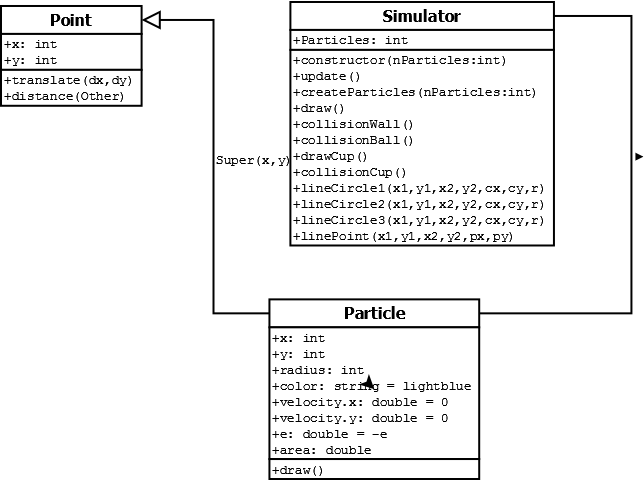
\includegraphics[width=\textwidth]{images/Diagram1.png}
	\caption{UML diagram (kör)}
	\label{fig:dia1}
\end{figure}


Jól látható, hogy a Particle osztály, a Point osztály leszármazottja, 2 származtatott metódussal.
Mindegyik osztály tartalmaz attribútumokat és műveleteket is.



\begin{figure}[h]
	\centering
	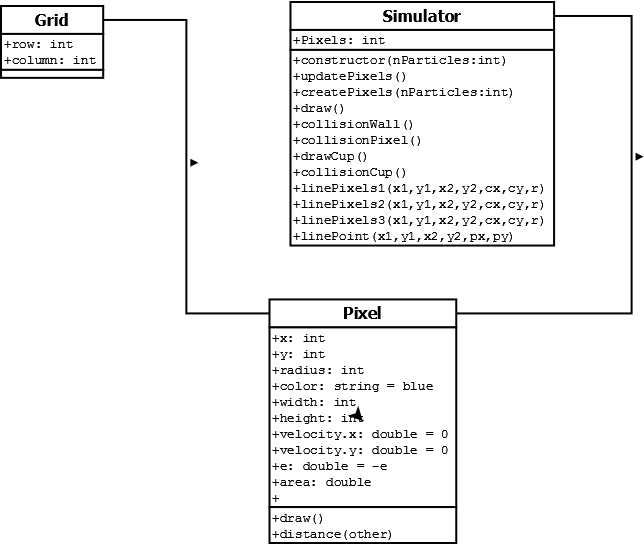
\includegraphics[width=\textwidth]{images/Diagram2.png}
	\caption{UML diagram (négyzet)}
	\label{fig:dia2}
\end{figure}


Itt is jól láthatóak a kapcsolatok az osztályok között. Ebben az esetben viszont nem mindegyik osztály tartalmaz műveleteket, de attribútumokat igen. 


